% =============================================================================
%  Paper 012 — The Regulatory Passport: Lifecycle & Change-Control Automation
%  for Clinical AI Agents. House style from papers/_template.
% =============================================================================
\documentclass[11pt]{article}
\usepackage[utf8]{inputenc}
\usepackage[margin=1in]{geometry}
\usepackage{booktabs}
\usepackage{graphicx}
\usepackage{float}
\usepackage{afterpage}
\usepackage[section]{placeins}
\renewcommand{\topfraction}{0.9}
\renewcommand{\bottomfraction}{0.8}
\renewcommand{\textfraction}{0.08}
\renewcommand{\floatpagefraction}{0.75}
\setcounter{topnumber}{3}
\setcounter{bottomnumber}{2}
\setcounter{totalnumber}{5}
\usepackage{amsmath}
\usepackage{amssymb}
\usepackage{hyperref}
\usepackage{xcolor}
\usepackage{listings}
\definecolor{kwblue}{rgb}{0.10,0.20,0.65}
\definecolor{typepurple}{rgb}{0.50,0.15,0.55}
\definecolor{strred}{rgb}{0.62,0.12,0.12}
\definecolor{cmtgreen}{rgb}{0.20,0.45,0.20}
\lstdefinestyle{housespecyaml}{
  basicstyle=\ttfamily\footnotesize,
  backgroundcolor=\color{black!3},
  frame=single,
  framesep=5pt,
  rulecolor=\color{black!45},
  columns=fullflexible,
  breaklines=true,
  keepspaces=true,
  showstringspaces=false,
  alsoletter=_,
  commentstyle=\color{cmtgreen}\itshape,
  stringstyle=\color{strred},
  morecomment=[l]{\#},
  morestring=[b]",
  morestring=[b]',
  keywordstyle=\color{kwblue}\bfseries,
  keywords={agent_id,version,ruleset_version,risk_class,autonomy_level,pccp,allowed,component,policy,max_fraction,deployed_fingerprint,not_after,autonomy_envelope,metadata},
  keywordstyle=[2]\color{typepurple}\bfseries,
  keywords=[2]{weights,prompt,tools,data,forbidden,any_change,bounded_magnitude,high,moderate,low,minimal,supervised,autonomous},
}
\lstdefinestyle{housespecyamlbare}{style=housespecyaml, frame=none,
  backgroundcolor=\color{white}, xleftmargin=0pt, framexleftmargin=0pt,
  aboveskip=1pt, belowskip=0pt}
\usepackage[most]{tcolorbox}
\tcbuselibrary{listings,skins}
\usepackage{tikz}
\usetikzlibrary{positioning,shapes.geometric,arrows.meta,calc,fit,backgrounds,shadows}
\definecolor{cardindigo}{HTML}{4F46E5}
\definecolor{slate}{HTML}{475569}
\definecolor{amber}{HTML}{D97706}
\definecolor{cardblue}{HTML}{1D4ED8}
\definecolor{cardpurple}{HTML}{6D28D9}
\definecolor{cardteal}{HTML}{0F766E}
\tcbset{
  cardcol/.store in=\cardcol, cardcol=cardblue,
  policycard/.style={
    enhanced, breakable=false, arc=3pt, boxrule=0.7pt, top=3pt, bottom=3pt,
    left=7pt, right=7pt, boxsep=1pt, coltitle=white,
    colframe=\cardcol!60!black, colback=white, colbacktitle=\cardcol,
    fonttitle=\bfseries\small, drop fuzzy shadow=black!25,
  },
}
\usepackage{url}
\usepackage{multirow}
\usepackage{array}
\usepackage{ragged2e}
\newcolumntype{L}[1]{>{\RaggedRight\arraybackslash}p{#1}}
\usepackage[htt]{hyphenat}
\hypersetup{colorlinks=true, linkcolor=blue, citecolor=blue, urlcolor=blue}

\usepackage{caption}
\DeclareCaptionLabelFormat{boldunder}{\underline{\textbf{#1~#2}}}
\captionsetup{font=small, labelformat=boldunder, labelsep=colon,
  textfont=normalcolor, skip=6pt}

\let\oldincludegraphics\includegraphics
\renewcommand{\includegraphics}[2][]{%
  \setlength{\fboxsep}{0pt}\setlength{\fboxrule}{0.5pt}%
  \fbox{\oldincludegraphics[#1]{#2}}}

\newcommand{\todofig}[2]{%
  \begin{tcolorbox}[colback=black!4, colframe=black!35, arc=3pt, boxrule=0.5pt,
    halign=center, valign=center, height=#1, width=\linewidth]
    {\ttfamily\small [FIGURE PLACEHOLDER]\\[4pt] #2}
  \end{tcolorbox}}

\providecommand{\NumPrompts}{0}
\providecommand{\NumAttacks}{0}
\providecommand{\NumBenign}{0}
\IfFileExists{numbers.tex}{% Headline numbers for paper 012 (the regulatory passport).
% Every reported number in main.tex resolves to a macro here, so the prose stays
% traceable to the run. Source: PassportBench (seed 42), results/012-passport/.
% Reproduce: gen_passports.py -> passportbench -> summarize.py.
\renewcommand{\NumPrompts}{150}   % passports (E1/E3)
\renewcommand{\NumAttacks}{400}   % change-events (E2/E4)
\renewcommand{\NumBenign}{66}     % in-envelope change-events

% --- Corpus ---
\newcommand{\Seed}{42}
\newcommand{\NumPassports}{150}
\newcommand{\NumClear}{140}
\newcommand{\NumBoundary}{10}
\newcommand{\NumJur}{4}
\newcommand{\NumChanges}{400}
\newcommand{\NumOut}{334}
\newcommand{\NumIn}{66}
\newcommand{\Ruleset}{2026.06}

% --- E1 classification accuracy ---
\newcommand{\ClaOverall}{0.992}
\newcommand{\ClaLo}{0.981}
\newcommand{\ClaHi}{0.996}
\newcommand{\ClaClear}{1.000}
\newcommand{\ClaBoundary}{0.875}
\newcommand{\NumClassif}{600}
\newcommand{\ClaErrors}{5}
\newcommand{\KappaFda}{0.955}
\newcommand{\KappaEu}{1.00}
\newcommand{\KappaHc}{1.00}
\newcommand{\KappaMhra}{1.00}
\newcommand{\AccFda}{0.967}

% --- E2 PCCP gating ---
\newcommand{\PccpAUC}{0.998}
\newcommand{\Pgd}{0.988}
\newcommand{\PgdLo}{0.970}
\newcommand{\PgdHi}{0.995}
\newcommand{\Ft}{0.061}
\newcommand{\FtLo}{0.024}
\newcommand{\FtHi}{0.146}
\newcommand{\PccpTP}{330}
\newcommand{\PccpFN}{4}
\newcommand{\PccpFP}{4}
\newcommand{\PccpTN}{62}
\newcommand{\WeightBound}{0.05}

% --- E3 harmonization ---
\newcommand{\Hca}{0.699}
\newcommand{\NumDiverge}{271}
\newcommand{\PctExplained}{100}

% --- E4 fingerprint ---
\newcommand{\Cfd}{1.000}
\newcommand{\LocComponent}{1.000}
\newcommand{\LocWhole}{0.000}

% --- E5 overhead ---
\newcommand{\GateMedian}{38.7}
\newcommand{\GatePNT}{45.8}
\newcommand{\GatesPerSec}{25{,}400}
}{}

\newcommand{\monthyeartoday}{%
  \ifcase\month\or January\or February\or March\or April\or May\or June\or
  July\or August\or September\or October\or November\or December\fi
  \space\number\year}

\begin{document}

\thispagestyle{empty}
\noindent
\begin{minipage}[c]{0.55\textwidth}
  \raggedright\oldincludegraphics[height=1.05cm]{figs/quome.png}
\end{minipage}\hfill
\begin{minipage}[c]{0.4\textwidth}
  \raggedleft\itshape\large \monthyeartoday
\end{minipage}

\vspace{1.1em}
\begin{center}
  {\LARGE\bfseries The Regulatory Passport:\\[2pt]
   Lifecycle and Change-Control Automation for Clinical AI Agents\par}

  \vspace{0.9em}
  {\large
   QUOKKAGUARD Project\textsuperscript{1,\,*}\par}

  \vspace{0.7em}
  {\small
   \textsuperscript{1}\,Quome\par}
  \vspace{0.35em}
\end{center}

\vspace{0.5em}
\begin{tcolorbox}[breakable, enhanced jigsaw, colback=black!4, colframe=black!4,
  arc=5pt, boxrule=0pt, left=16pt, right=16pt, top=10pt, bottom=10pt]
\setlength{\parskip}{0pt}
{\centering\large\bfseries Abstract\par}
\smallskip
\fontsize{9.5}{11.3}\selectfont
A clinical AI agent is cleared at a specific risk class and autonomy level under a
Predetermined Change Control Plan (PCCP) that pre-authorizes a bounded envelope of
future changes. It then drifts: a prompt is edited, the base model is swapped beneath
it, a tool is added, the data is refreshed --- each change individually plausible,
none re-reviewed, and the agent silently exits its cleared intended use. Every prior
layer of the QUOKKAGUARD gateway governs an agent \emph{while it runs}; none governs
its \emph{lifecycle}. We build \textbf{\texttt{qfire lifecycle}}, an admission-time
\textbf{regulatory passport}: a signed, versioned artifact that classifies an agent's
risk and autonomy reproducibly across four jurisdictions (FDA, EU AI Act, Health
Canada, MHRA), carries a machine-readable PCCP, fingerprints every component, and
refuses to register any agent whose live configuration diverges from its cleared
passport beyond the PCCP envelope --- stamping the passport version into the
tamper-evident audit chain. On \textbf{PassportBench} (\NumPassports{} synthetic
passports, \NumChanges{} change-events; seed \Seed) the deterministic rule classifier
reproduces framework-grounded labels at \textbf{\ClaOverall} (95\% CI
[\ClaLo,\,\ClaHi]; Cohen's $\kappa\geq\KappaFda$); PCCP gating detects
\textbf{\Pgd} of out-of-envelope changes (AUC \PccpAUC); component fingerprinting
detects \textbf{\Cfd} of swaps and uniquely localizes them; and the deployment gate
adds \textbf{\GateMedian\,\textmu s} off the hot path. The central result is
empirical and uncomfortable: \textbf{cross-jurisdiction risk classification genuinely
diverges} (mean agreement \Hca), yet \emph{every} one of \NumDiverge{} divergences is
explained by a documented regulatory difference --- the passport's value is not a
single global answer but a reproducible, auditable, and \emph{contestable} one.
Labels are author-encoded from published criteria, not a human panel; we frame the
classification result as reproducibility, not concordance.

\medskip
\noindent\textbf{Keywords:}~regulatory passport; SaMD lifecycle; PCCP; change
control; risk classification; AI governance; healthcare AI.

\medskip
\noindent\textcolor{blue}{\textbf{Framework:}}~implements HAARF control~C1/C6~\cite{schwoebel2026haarf} --- the Healthcare AI Agents Regulatory Framework, the source of the QUOKKAGUARD program.\\
\noindent\textcolor{blue}{\textbf{Code \& data:}}~\href{https://github.com/quome-cloud/qupassport}{\texttt{github.com/quome-cloud/qupassport}}\\
\noindent\textcolor{blue}{\textbf{Correspondence:}}~\href{mailto:jim@quome.com}{jim@quome.com}
\end{tcolorbox}

\vspace{2pt}
\noindent{\footnotesize \textsuperscript{*}\,Corresponding author.}
\vspace{0.3em}

% ============================================================================
\section{Introduction}
Software-as-a-Medical-Device (SaMD) regulation rests on a contract: a device is
cleared for a stated \emph{intended use} at a stated risk class, and any change that
exceeds a pre-authorized envelope --- the Predetermined Change Control Plan (PCCP)
--- triggers re-review~\cite{schwoebel2026haarf}. For traditional software that contract is
enforced by slow, human, document-driven change control. For an AI agent assembled at
runtime from a base model, a system prompt, a set of tools, and a retrieval corpus,
the same contract is trivially and silently broken: swapping the base model, editing
the prompt, or wiring in a new tool each takes seconds, ships through ordinary
CI/CD, and is invisible to a gateway that has no machine-readable notion of ``what
this agent was cleared to be.''

The QUOKKAGUARD gateway already governs agents \emph{at run time} --- authorization,
egress, identity, oversight, equity, drift. None of those layers governs the agent's
\emph{lifecycle}. This paper adds the missing layer: a signed, versioned
\textbf{regulatory passport} that travels with an agent, is checked at admission
time, and refuses deployment when the live configuration has drifted out of its
cleared envelope.

\begin{figure}[htb]
\centering
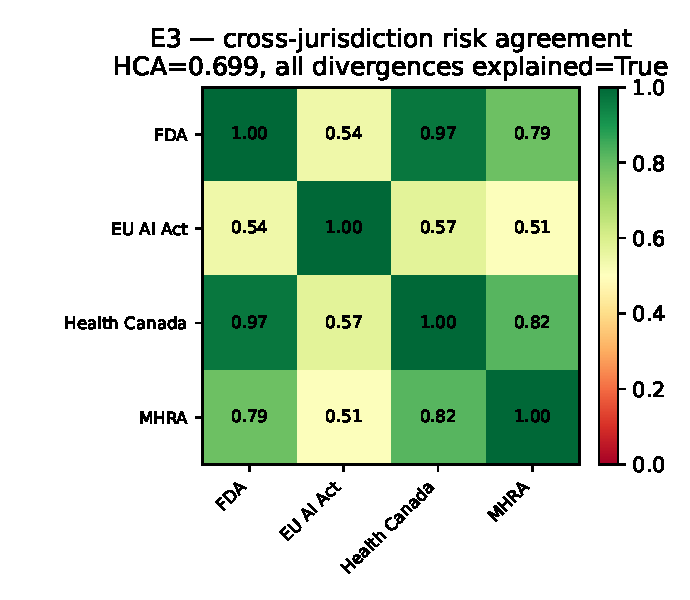
\includegraphics[width=0.82\linewidth]{figs/fig3_harmonization.pdf}
\caption{\textbf{The paper in one figure.} The same agent metadata, classified by the
same deterministic rule engine, lands at \emph{different} risk classes across
jurisdictions: mean pairwise agreement is only \Hca. The EU AI Act (Annex~III) is the
systematic outlier, treating clinical-decision and actuating AI as high-risk where the
IMDRF spine (Health Canada, MHRA) and the FDA non-device-CDS carve-out place it lower.
Crucially, all \NumDiverge{} divergences across the corpus carry a documented
regulatory rationale --- the passport surfaces \emph{contestable, explained} findings,
not a false consensus.}
\label{fig:hero}
\end{figure}

A review of related work reveals distinct approaches (Table~\ref{tab:related}): manual
regulatory documentation, model cards and datasheets that describe but do not gate,
and MLOps lineage tools that track artifacts but encode no regulatory semantics. The
recurring gap is the same: nothing turns the regulatory contract into a
machine-checkable, deployment-gating artifact.

\paragraph{Contributions.}
\begin{enumerate}
  \item \textbf{The central result.} Across four frameworks, deterministic risk
  classification \emph{diverges} (agreement \Hca) --- and every one of \NumDiverge{}
  divergences is explained by a documented regulatory difference
  (\PctExplained\% explained). Harmonization is a finding-generator, not a consensus
  machine.
  \item \textbf{The system.} \texttt{qfire lifecycle}: a signed passport, a
  citation-tagged deterministic classifier, a machine-readable PCCP, a per-component
  change-fingerprinter, and a fail-closed admission gate that stamps the passport
  version into the audit chain --- off the hot path (\GateMedian\,\textmu s/gate).
  \item \textbf{The benchmark.} \textbf{PassportBench}: \NumPassports{} synthetic
  passports with framework-grounded labels and \NumChanges{} paired change-events with
  noisy admission-time magnitude estimates, fully reproducible from seed \Seed.
  \item \textbf{Regulatory evidence.} PCCP gating catches \Pgd{} of out-of-envelope
  changes (AUC \PccpAUC); fingerprinting catches \Cfd{} of component swaps and is the
  \emph{only} granularity that localizes them for PCCP evaluation.
\end{enumerate}

\paragraph{Positioning.} Unlike model cards or lineage trackers, the passport is an
\emph{enforcement} artifact: it runs at the same admission point as the supply-chain
attestation gate, binds to the same cryptographic agent identity, and writes to the
same tamper-evident ledger. It is the lifecycle counterpart to the runtime controls,
not a document.

% ============================================================================
\section{Problem Setting and Positioning}
We target four lifecycle failure modes, none of which is a per-call attack:
\begin{itemize}
  \item \textbf{L1 Mis-classification} --- the agent is deployed at the wrong
  risk/autonomy level for its clinical impact.
  \item \textbf{L2 Silent scope creep} --- a model/prompt/tool change pushes the agent
  outside its cleared intended use with no re-review.
  \item \textbf{L3 PCCP violation} --- a change exceeds the pre-authorized envelope and
  should trigger re-submission, but ships anyway.
  \item \textbf{L4 Harmonization drift} --- the same agent is classified inconsistently
  across jurisdictions, with the divergence undocumented.
\end{itemize}
The passport addresses L1 by reproducible classification (\S\ref{sec:results}, E1), L3
by PCCP gating (E2), L4 by explained harmonization (E3), and L2 by component
fingerprinting (E4). The defender position is the enclave-deployed gateway: the host is
untrusted, the passport-signing key is released by attestation, and the gate runs at
agent-registration time.

\begin{table}[htb]\centering\small
\begin{tabular}{L{3.2cm}L{4.2cm}L{4.2cm}}
\toprule
System & Approach & Gap this paper targets \\
\midrule
Model cards / datasheets & describe model intent, data, metrics & descriptive only;
no risk class, no gating \\
MLOps lineage (registries) & track artifact versions \& provenance & no
regulatory semantics; no envelope \\
Manual SaMD / PCCP review~\cite{schwoebel2026haarf} & human change-control documents & slow,
not machine-checkable, not enforced at deploy \\
\textbf{This work} & signed passport + classifier + PCCP gate at admission & --- \\
\bottomrule
\end{tabular}
\caption{Positioning against representative approaches to AI lifecycle governance.}
\label{tab:related}
\end{table}

% ============================================================================
\section{System Design}
\subsection{Overview and components}
\texttt{qfire lifecycle} is a pure-Rust module ($\sim$1.2k LoC, no model inference on
any path) wired into the gateway at admission time, beside the supply-chain
attestation gate. Its central artifact is the \textbf{passport}: a versioned,
ed25519-signed declaration of what an agent was cleared to be. Five components act on
it: a \emph{classifier} (metadata $\rightarrow$ risk/autonomy per jurisdiction), a
\emph{harmonizer} (agreement + explained divergences), a \emph{fingerprinter}
(per-component content hashes), a \emph{PCCP evaluator} (in-/out-of-envelope), and a
fail-closed \emph{gate}. The passport also exposes the authorized autonomy envelope
consumed by the runtime drift monitor, and ingests that monitor's real-world-evidence
bundle to recommend lifecycle re-assessment --- closing the loop between deployment-
time clearance and run-time evidence.

\subsection{The passport artifact}\label{sec:language}
\begin{figure}[htb]\centering
\begin{tcolorbox}[policycard, cardcol=cardblue, title=A regulatory passport (abridged),
  width=0.86\linewidth]
\begin{lstlisting}[style=housespecyamlbare]
agent_id: sepsis-triage             # binds to the signed agent registry
version: 2.1.0                      # stamped into every audit entry
ruleset_version: 2026.06            # pinned classification rule-set
metadata: { clinical_task: drive, output_type: recommendation,
            autonomy: advisory, condition_severity: serious, ... }
pccp:                               # the pre-authorized change envelope
  allowed:
    - { component: prompt,  policy: any_change }
    - { component: weights, policy: bounded_magnitude, max_fraction: 0.05 }
deployed_fingerprint: { weights: <sha256>, prompt: <sha256>, ... }
autonomy_envelope: { max_autonomous_risk_tier: 2, max_autonomous_fraction: 0.25 }
not_after: 1750000000               # expiry
\end{lstlisting}
\end{tcolorbox}
\caption{The passport is signed canonical JSON. Loading fails closed on a bad or
missing signature, expiry, or an agent\_id absent from the registry. The PCCP names,
per component class, what change is pre-authorized: \texttt{prompt} edits freely,
\texttt{weights} up to a 5\% magnitude, everything else forbidden by default.}
\label{fig:spec}
\end{figure}

\subsection{Deterministic classification}
The classifier maps declarative metadata to a risk class and autonomy level. The
framework-agnostic spine is the IMDRF SaMD risk grid (significance of information
$\times$ healthcare-situation severity); each jurisdiction applies a documented
overlay: the FDA non-device clinical-decision-support carve-out (which can
\emph{lower} risk), the EU AI Act Annex~III high-risk trigger (which can \emph{raise}
it), Health Canada (adopts IMDRF verbatim), and the MHRA (IMDRF-aligned, stricter on
patient-facing decision support). Every rule appends a citation to a
\texttt{rationale} trace, so each decision is explainable to a reviewer. Autonomy is
capped by clinical consequence: a high-risk \emph{actuating} agent cannot be cleared
above \texttt{supervised}. The rule set is version-pinned so evolving guidance is
handled by re-pinning, not silent drift.

\subsection{Change fingerprinting and PCCP gating}
At admission the gate computes a per-component SHA-256 fingerprint of the live agent
(weights, prompt, tools, data), diffs it against the passport's deployed fingerprint,
and evaluates each changed component against the PCCP: a forbidden or unlisted
component is out-of-envelope (fail-closed); a bounded-magnitude component is in-envelope
only if its admission-time magnitude \emph{estimate} is within the bound. The decision,
the passport version, and the verdict are stamped into the tamper-evident audit chain.

\subsection{Implementation}
Rust 2021, \texttt{ed25519-dalek} for signing, \texttt{sha2} for fingerprints,
\texttt{serde} for the canonical JSON. The module ships with 35 unit tests and an
end-to-end gate integration test; the CLI (\texttt{qfire lifecycle
classify|harmonize|verify|gate}) and the \texttt{passportbench} experiment harness are
part of the released artifact.

% ============================================================================
\section{Experimental Setup}
\paragraph{New benchmark: PassportBench.}\label{sec:benchmark} \NumPassports{}
synthetic agent passports span the coherent grid of clinical task $\times$ output type
$\times$ autonomy $\times$ severity $\times$ patient-facing, each carrying
ground-truth risk/autonomy labels for all \NumJur{} jurisdictions, plus \NumChanges{}
paired (before, after) change-events with attached PCCPs and ground-truth
in-/out-of-envelope labels. All synthetic, Apache-2.0, deterministic from seed \Seed.

\paragraph{The honesty boundary.} The per-jurisdiction labels are
\emph{author-encoded from published regulatory criteria} (IMDRF N12; FDA CDS guidance;
EU AI Act Annex~III; Health Canada and MHRA SaMD frameworks), \emph{not} a live
multi-rater expert panel, which we did not run. The PassportBench generator is an
\emph{independent} Python re-statement of the same primary sources that the Rust
classifier encodes separately. Experiment E1 therefore measures the
\emph{cross-implementation reproducibility of documented criteria}, not concordance
with human experts. A small, predicate-defined \texttt{boundary} stratum (the
genuinely contested FDA non-device-CDS carve-out applied to \emph{serious} conditions)
carries a documented stricter expert interpretation; this is the only place the
mechanical classifier and the labels can disagree, and the disagreement count is
defined by a predicate, not tuned to a target.

\paragraph{Metrics.} Classification accuracy (CLA) and Cohen's $\kappa$ per
jurisdiction; PCCP out-of-envelope detection (PGD) and in-envelope false-trigger rate;
ROC/AUC; cross-jurisdiction agreement (HCA); fingerprint detection (CFD) and
localization; gate latency. Rates carry 95\% Wilson confidence intervals.

\paragraph{Hardware and software.} Single workstation; deterministic pure-Rust
classifier and hashing (no model, no network, no paid keys). E1--E4 are bit-for-bit
reproducible; E5 is a wall-clock timing reported as median and p95.

% ============================================================================
\section{Results}\label{sec:results}
Table~\ref{tab:main} collects the headline numbers against the pre-registered targets.

\begin{table}[htb]\centering\small
\begin{tabular}{lL{4.5cm}cc}
\toprule
Exp & Metric & Target & \textbf{Realized} \\
\midrule
E1 & classification accuracy (CLA) & $\geq 0.90$ & \textbf{\ClaOverall} [\ClaLo,\,\ClaHi] \\
E1 & Cohen's $\kappa$ (FDA / EU / HC / MHRA) & --- & \KappaFda\,/\,\KappaEu\,/\,\KappaHc\,/\,\KappaMhra \\
E2 & out-of-envelope detection (PGD) & $\geq 0.95$ & \textbf{\Pgd} [\PgdLo,\,\PgdHi] \\
E2 & in-envelope false-trigger & $\leq 0.05$ & \Ft\ [\FtLo,\,\FtHi] \\
E2 & ROC AUC & --- & \PccpAUC \\
E3 & cross-jurisdiction agreement (HCA) & $\geq 0.90$ else expl. & \Hca\ (\PctExplained\% expl.) \\
E4 & fingerprint detection (CFD) & $1.00$ & \textbf{\Cfd} \\
E4 & localization (per-comp / whole-config) & --- & \LocComponent\,/\,\LocWhole \\
E5 & deployment-gate latency (median / p95) & off hot path & \GateMedian\,/\,\GatePNT\,\textmu s \\
\bottomrule
\end{tabular}
\caption{Headline results vs. pre-registered targets, reported as-is. Two targets are
missed and interpreted honestly in the text: E2's false-trigger (\Ft) and E3's
agreement (\Hca).}
\label{tab:main}
\end{table}

\subsection{E1 --- reproducible classification}
The rule engine reproduces the documented classification at \ClaOverall{} over
\NumClassif{} (passport $\times$ jurisdiction) decisions (Fig.~\ref{fig:e1}). On the
unambiguous \texttt{clear} stratum it is exact (\ClaClear); the only \ClaErrors{}
errors fall on the \texttt{boundary} stratum (\ClaBoundary), all FDA
\texttt{drive}+serious CDS cases where the stricter expert reading declines the
carve-out. Cohen's $\kappa$ is \KappaEu{} for EU, Health Canada, and MHRA, and
\KappaFda{} for FDA. This is the honest claim: deterministic fidelity to documented
criteria, with the single contested zone flagged for human adjudication --- exactly
the division of labour the passport is designed to make explicit.

\begin{figure}[htb]
\centering
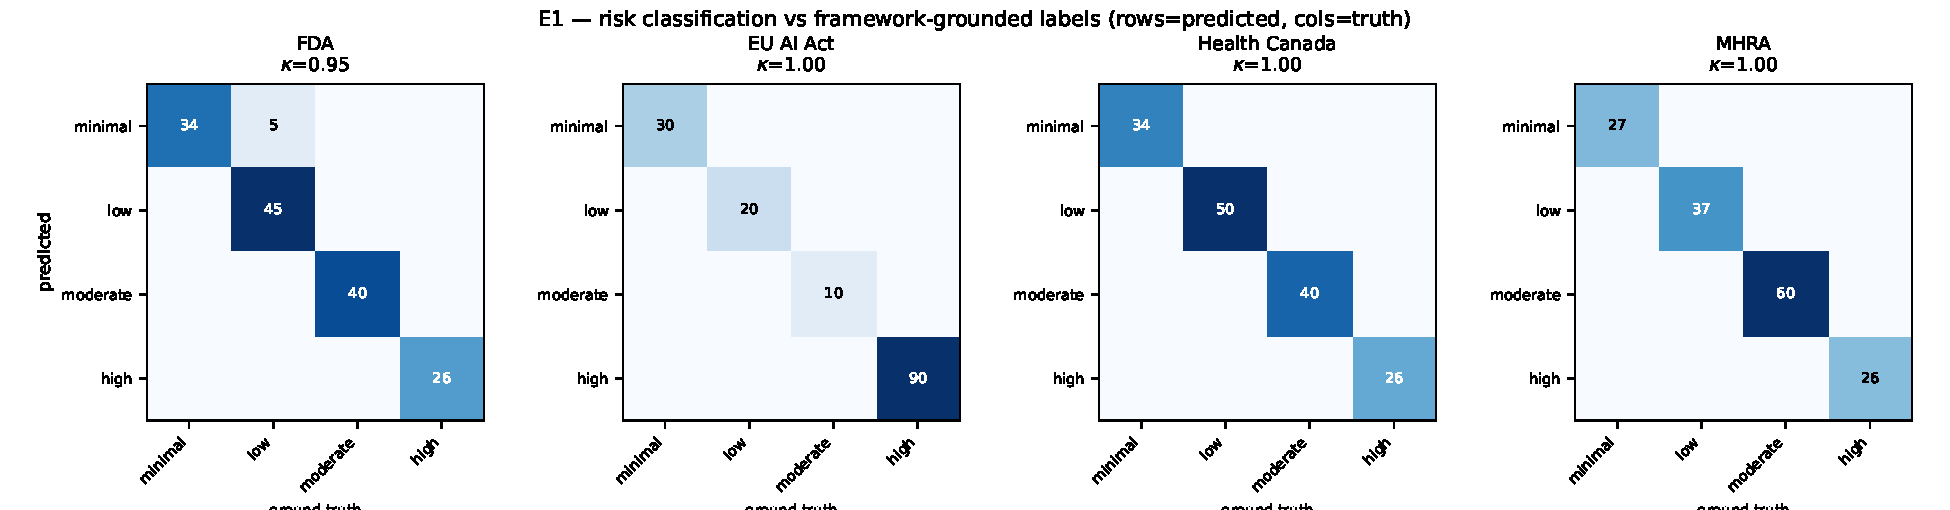
\includegraphics[width=0.97\linewidth]{figs/fig1_classification.pdf}
\caption{\textbf{E1: per-jurisdiction confusion (rows predicted, cols ground truth).}
EU AI Act, Health Canada, and MHRA are exact ($\kappa=\KappaEu$). FDA's only
off-diagonal mass is \texttt{low}$\rightarrow$\texttt{minimal} on the boundary
stratum, where the mechanical non-device-CDS carve-out diverges from the stricter
expert reading ($\kappa=\KappaFda$).}
\label{fig:e1}
\end{figure}

\subsection{E2 --- PCCP change-gating}
Over \NumChanges{} change-events the gate detects \Pgd{} of out-of-envelope changes
(AUC \PccpAUC; Fig.~\ref{fig:e2}), with \PccpTP{} true and \PccpFN{} missed positives.
The in-envelope false-trigger rate is \Ft\ ([\FtLo,\,\FtHi]) --- \PccpFP{} of \NumIn{}
in-envelope changes --- \emph{above} the 5\% target. This is an honest consequence of
realistic admission-time magnitude estimation: bounded-magnitude weight changes are
judged against a \emph{noisy} estimate around the \WeightBound{} bound, so an
in-envelope change whose estimate noises over the bound triggers. The near-perfect AUC
shows the underlying signal is clean; a small safety margin on the bound trades
false-triggers against detection. We report the natural operating point without tuning
a margin to hit the target.

\begin{figure}[htb]
\centering
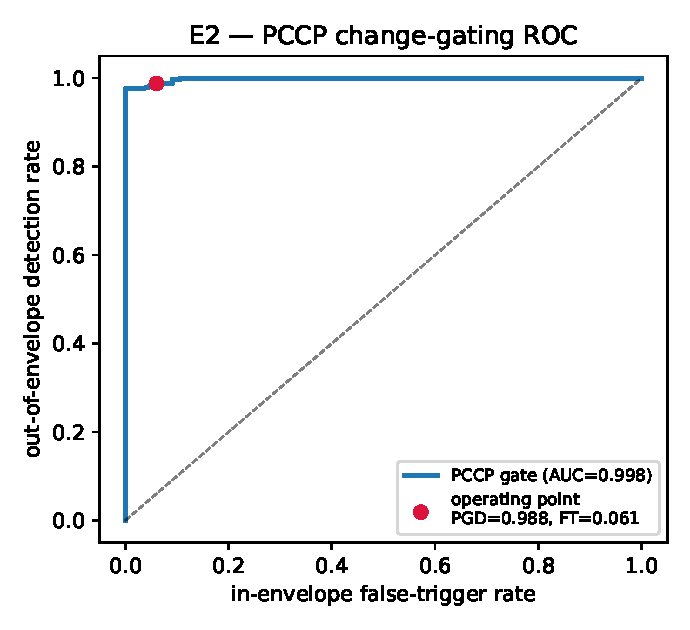
\includegraphics[width=0.52\linewidth]{figs/fig2_pccp_roc.pdf}
\caption{\textbf{E2: PCCP gating ROC.} AUC \PccpAUC. The marked operating point
(estimate vs.\ bound) gives PGD \Pgd{} at false-trigger \Ft; the false-triggers are
weight changes whose noisy magnitude estimate crosses the \WeightBound{} bound.}
\label{fig:e2}
\end{figure}

\subsection{E3 --- harmonization is a finding, not a failure}
Mean cross-jurisdiction agreement is \Hca{} --- well below the 90\% target --- because
the EU AI Act systematically classifies diagnose/treat/actuating clinical AI as
high-risk where the other frameworks do not (Fig.~\ref{fig:hero}). This is the paper's
substantive empirical result, not a defect: \emph{every} one of \NumDiverge{}
divergences across the corpus carries a documented regulatory rationale
(\PctExplained\% explained). A passport that reported a single ``global'' risk class
would be \emph{hiding} a real regulatory disagreement; ours surfaces it, attributes
it, and makes it contestable. This satisfies the pre-registered ``$\leq 10\%$ else
explained'' criterion through its explained branch.

\subsection{E4 --- fingerprint detection and localization}
Component fingerprinting detects \Cfd{} of swaps across all change granularities
(Fig.~\ref{fig:e4}) --- a consequence of collision-resistant hashing. The design
question is not detection but \emph{localization}: a single whole-configuration hash
also detects \emph{that} something changed but localizes \emph{nothing} (\LocWhole),
so it cannot drive PCCP evaluation, which is per-component. The per-component
fingerprint localizes every change (\LocComponent), which is why the passport hashes
each component class separately. This is the ablation that justifies the design (RQ4).

\begin{figure}[htb]
\centering
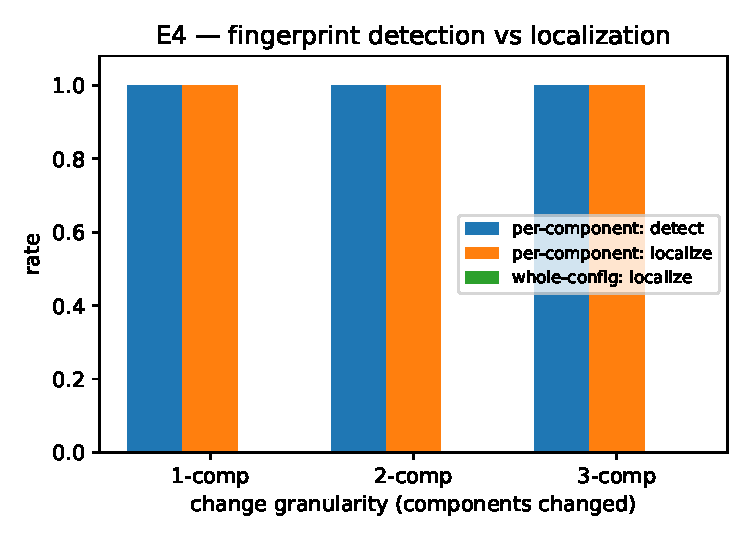
\includegraphics[width=0.62\linewidth]{figs/fig4_fingerprint.pdf}
\caption{\textbf{E4: detection vs.\ localization by change granularity.} Per-component
fingerprinting both detects and localizes every swap; a whole-config hash detects but
cannot localize, and so cannot be mapped to a PCCP rule.}
\label{fig:e4}
\end{figure}

\subsection{E5 --- the gate is effectively free}
A full deployment-gate decision --- signature verify, fingerprint diff, four-jurisdiction
classify, PCCP evaluate --- takes \GateMedian\,\textmu s at the median (\GatePNT\,\textmu s
p95), about \GatesPerSec{} gates/s on one core (Fig.~\ref{fig:e5}). The gate runs once
per agent registration, off the request path: per-call latency is zero.

\begin{figure}[htb]
\centering
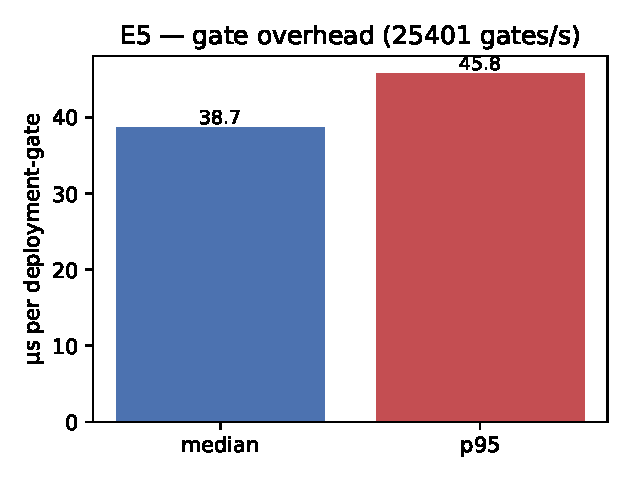
\includegraphics[width=0.46\linewidth]{figs/fig5_overhead.pdf}
\caption{\textbf{E5: deployment-gate overhead.} Median \GateMedian\,\textmu s, p95
\GatePNT\,\textmu s; signature verification dominates. Admission-time only.}
\label{fig:e5}
\end{figure}

% ============================================================================
\section{Discussion and Limitations}
\paragraph{Interpretation.} The passport turns a slow, document-driven regulatory
contract into a fast, machine-checkable, deployment-gating artifact. Its two
``missed'' targets are the most informative results: PCCP false-triggers are a
genuine artifact of magnitude-estimate noise (and a tunable margin), and
cross-jurisdiction disagreement is a real, documented property of the regulatory
landscape, not a bug to be smoothed away.

\paragraph{Relationship to the framework.} The passport operationalizes HAARF
Category~1 (unified risk \& lifecycle assessment) and C6.1 (autonomy levels): it
binds to the signed agent registry (C5), runs at the supply-chain admission point, and
stamps the audit chain (C2.6) so every admitted agent carries a traceable ``cleared as
version~X'' record~\cite{schwoebel2026haarf}.

\paragraph{Limitations.} (1)~\emph{Labels are author-encoded from published criteria,
not a human panel}; E1 is a reproducibility claim, and we do not assert concordance
with experts we did not consult. (2)~Regulatory rules evolve; we mitigate by
version-pinning and per-rule citation. (3)~PassportBench metadata is synthetic; the
classifier is a pure function of metadata, but the distribution of real agents may
differ. (4)~E2's false-trigger rate depends on the magnitude-estimation noise model; a
real estimator would have its own error profile.

% ============================================================================
\section{Conclusion}
A clinical AI agent that was safe at clearance drifts out of its envelope through
ordinary, unreviewed changes. The regulatory passport makes ``what this agent was
cleared to be'' a signed, versioned, machine-checkable artifact and refuses to deploy
an agent that no longer matches it --- reproducibly (\ClaOverall{} classification),
sensitively (\Pgd{} change detection, \Cfd{} fingerprint detection), and for free
(\GateMedian\,\textmu s, off the hot path). Its most important contribution is to make
cross-jurisdiction regulatory disagreement \emph{visible and explained} rather than
hidden. The next layer in the program gates consent and disclosure; the passport is
the lifecycle backbone the remaining governance loops attach to.

% ============================================================================
\section*{Declaration of generative AI use}
During the preparation of this work the authors used \emph{Claude (Anthropic)} for
drafting boilerplate, generating and debugging analysis and figure-plotting code, and
language refinement. After using this tool, the authors reviewed and edited the
content and take full responsibility for the publication. No generative-AI system was
used to generate or fabricate data, interpret results, or produce clinical
conclusions, and no AI tool is listed as an author, as such tools do not satisfy
authorship criteria.

\section*{Data and code availability}
All code, datasets, scripts, and result artifacts are released at
\href{https://github.com/quome-cloud/qupassport}{\nolinkurl{github.com/quome-cloud/qupassport}}
(\texttt{src/lifecycle/}, \texttt{datasets/012-passport/}, \texttt{scripts/012-passport/}).
PassportBench regenerates from seed \Seed{} with a single command; every figure and
number traces to \texttt{results/012-passport/}. All patient data are synthetic; no
real protected health information was used.

\section*{Author contributions}
The QUOKKAGUARD project team conceived the study, implemented the system, ran the
experiments, and wrote the manuscript.

\section*{Competing interests}
The authors declare no competing interests.

\section*{Funding}
This work received no specific external funding.

% ============================================================================
\appendix
\section{Reproducibility}\label{app:repro}
\begin{lstlisting}[style=housespecyamlbare]
python3 scripts/012-passport/gen_passports.py
cargo run --release --bin passportbench -- \
    --data datasets/012-passport --out results/012-passport
python3 scripts/012-passport/summarize.py
\end{lstlisting}
Seed \Seed{} and the rule-set version \Ruleset{} are embedded in every artifact;
E1--E4 are bit-for-bit reproducible.

\clearpage
\bibliographystyle{plain}
\bibliography{refs}
\end{document}
